% !TEX TS-program = pdflatex
% !TEX encoding = UTF-8 Unicode

% This is a simple template for a LaTeX document using the "article" class.
% See "book", "report", "letter" for other types of document.

\documentclass[11pt]{article} % use larger type; default would be 10pt

\usepackage[utf8]{inputenc} % set input encoding (not needed with XeLaTeX)

%%% Examples of Article customizations
% These packages are optional, depending whether you want the features they provide.
% See the LaTeX Companion or other references for full information.

%%% PAGE DIMENSIONS
\usepackage{geometry} % to change the page dimensions
\geometry{letterpaper} % or letterpaper (US) or a5paper or....
% \geometry{margin=2in} % for example, change the margins to 2 inches all round
% \geometry{landscape} % set up the page for landscape
%   read geometry.pdf for detailed page layout information

\usepackage{graphicx} % support the \includegraphics command and options

% \usepackage[parfill]{parskip} % Activate to begin paragraphs with an empty line rather than an indent

%%% PACKAGES
\usepackage{booktabs} % for much better looking tables
\usepackage{array} % for better arrays (eg matrices) in maths
\usepackage{paralist} % very flexible & customisable lists (eg. enumerate/itemize, etc.)
\usepackage{verbatim} % adds environment for commenting out blocks of text & for better verbatim
\usepackage{subfig} % make it possible to include more than one captioned figure/table in a single float
% These packages are all incorporated in the memoir class to one degree or another...

%%% HEADERS & FOOTERS
\usepackage{fancyhdr} % This should be set AFTER setting up the page geometry
\pagestyle{fancy} % options: empty , plain , fancy
\renewcommand{\headrulewidth}{0pt} % customise the layout...
\lhead{}\chead{}\rhead{}
\lfoot{}\cfoot{\thepage}\rfoot{}

%%% SECTION TITLE APPEARANCE
\usepackage{sectsty}
\allsectionsfont{\sffamily\mdseries\upshape} % (See the fntguide.pdf for font help)
% (This matches ConTeXt defaults)

%%% ToC (table of contents) APPEARANCE
\usepackage[nottoc,notlof,notlot]{tocbibind} % Put the bibliography in the ToC
\usepackage[titles,subfigure]{tocloft} % Alter the style of the Table of Contents
\renewcommand{\cftsecfont}{\rmfamily\mdseries\upshape}
\renewcommand{\cftsecpagefont}{\rmfamily\mdseries\upshape} % No bold!

%%% END Article customizations

\renewcommand\thesubsection{\alph{subsection})}

%%% The "real" document content comes below...
\usepackage[normalem]{ulem}

\title{Final Exam: SVD and the Netflix Problem}
\author{ Gregory \uline{Smetana} \\ID 1917370 \\ ACM 106a }
%\date{} % Activate to display a given date or no date (if empty),
         % otherwise the current date is printed 

\usepackage{fancyhdr}
\usepackage{lastpage}

\usepackage{../mcode}

\usepackage{mathtools}
\pagestyle{fancy}
\lhead{Gregory \uline{Smetana}}
\rhead{ID 1917370 }


\begin{document}


\maketitle

\section{Recommender systems and SVD}
Recommender systems or recommendation systems are broadly defined as algorithms used to predict the
rating an individual would assign to an item. For example, an online vendor may want to determine the
preferences of its users in order to recommend new products (and increase its sales). These preferences can
be thought of as being stored in a matrix with rows corresponding to items in the vendor’s catalogue and
columns corresponding to each user; the $(i, j)$th entry of this matrix would be the rating given to item $i$ by
user $j$. For example, the Netflix data set consists of a matrix with rows corresponding to movies in Netflix’s
catalogue, columns indexed by users and entries corresponding to a user rating of a particular movie on an
integer scale from one to five.

Unfortunately, most entries of this preference matrix are unknown in general; many, if not all, users will
not have rated every item in the catalogue. The goal of a recommender system is to obtain a good estimate
of the unknown entries of this preference matrix. This is a special case of the matrix completion problem:
given partially known matrix $M$ , compute the unknown entries of $M$ . Clearly, this problem is absurdly
underdetermined; for example, without any additional assumptions, any value between one and five can be
assigned to each unknown entry of the Netflix matrix. One classical approach to the matrix completion
problem is to place some additional assumption on the matrix $M$ to be completed, e.g., that $M$ is low-rank,
and perform regularization to choose a particular solution. This is not an unreasonable assumption regarding
the structure of preference matrices. For example, it is widely theorized and/or assumed that individual
users in the Netflix matrix can be represented as a linear combination of a relatively small number of
eigencustomers, whose behaviour represent canonical preferences. For example, one eigencustomer may be
a user who only watches documentaries, another is someone who only enjoys comedies, etc. Similarly, any
movie can be represented as a combination of eigenmovies. Although there may be many canonical users or
catalogue items, it is highly likely that the number of such users or items should be much smaller than the
dimensions of the preference matrix (on the order of dozens versus tens of thousand of movies and millions
of users in the case of the Netflix matrix). This corresponds to the preference matrix having very small rank
(relative to its dimension).

This assumption leads to a natural formulation of the problem as an underdetermined linear system with
matrix rank used for regularization. Unfortunately, this requires the solution of an intractable optimization
problem and the methods for approximately solving it are well beyond the scope of this course; however, if
you are interested this may be covered in ACM 113: Introduction to Optimization. Instead, we will use a
classical technique based on singular value decomposition of the preference matrix to obtain our predicted
user ratings. This heuristic follows two steps. In the first, values are assigned to the unknown entries of
the preference matrix. For example, if the $(i, j)$ entry is unknown, then we may assign a value by taking a
combination of the average rating for movie $i$ or the average rating by user $j$. Once the unknown entries
have been assigned a value, we obtain a rank-$k$ prediction matrix using the singular value decomposition of
the preference matrix (with filled in entries). The use of low-rank matrices to identify a low-dimensional set
of latent variables explaining variance also plays a significant role in the analysis of (incomplete) scientific
data, especially that arising from applications in geophysics, and is closely related to principal component
analysis; this will likely be discussed at length in ACM/ESE 118: Methods in Applied Statistics and Data
Analysis.

\section{Description of partial SVD algorithm}

The outline of the partial SVD algorithm is similar to the full SVD algorithm

\begin{enumerate}
\item Form matrix $A^T A$
\item Compute partial eigendecomposition $A^T A \approx V_k D_k V_k^T$
\item Let $\Sigma_k = D_k^{1/2}$
\item Solve the system $U_k \Sigma_k  = A_k V_k$ for the matrix of left singular vectors $U_k$.
\end{enumerate}

\subsection{Partial eigendecomposition of $A^T A$}

To compute the partial eigendecomposition of the symmetric matrix $A^T A$ in Step 2, the Lanczos algorithm in floating point arithmetic of Demmel Algorithm 7.2 is used:

\begin{equation}
\begin{split}
 &q_1 = b / \|b\|_2, \beta_0 = 0, q_0 = 0\\
&\text{for } j = 1 \text{ to } k\\
&\quad z = A q_k\\
& \quad \alpha_j = q_j^T z\\
& \quad z = z-\sum_{i=1}^{j-1} (z^T q_i)q_i \\
& \quad z = z-\sum_{i=1}^{j-1} (z^T q_i)q_i \\
& \quad \beta_j = \|z\|_2\\
& \quad \text{if } \beta_j = 0,  \text{quit}\\
& \quad q_{j+1} = z / \beta_j\\
& \quad \text{Compute eigenvalues, eigenvectors, and error bounds of } T_k\\
& \text{end}
\end{split}
\end{equation}

The $z = z-\sum_{i=1}^{j-1} (z^T q_i)q_i $  steps are to reorthogonalize after loss of orthogonality in floating point arithmetic. If the Lanczos vectors are not kept orthogonal, there may be multiple copies of converged Ritz values.

The algorithm was said to be converged when
\begin{equation}
| \beta_n | | v_k (n) | < tol
\end{equation}

\subsection{Eigenvalues and eigenvectors of $T_k$}

In computing the eigenvalues and eigenvectors of $T_k$ during the Lanczos iteration, QR iteration with a shift was used:
\begin{equation}
\begin{split}
&i = 0\\
&\text{repeat}\\
&\quad \text{Choose a shift }\sigma_i \\
& \quad \text{Factor }A_i - \sigma_i I = Q_i R_i \\
& \quad A_{i+1} = Q_i^T A_i Q_i \\
& \quad i = i+1 \\
&\text{Until convergence}
\end{split}
\end{equation}

Convergence was defined as the off-diagonal entries of $A$ being smaller than $tol$.

\subsubsection{QR iteration shift}
The QR iteration used Wilkinson's shift. This shift is the eigenvalue of the lower right $2 \times 2$ submatrix of $A_i$
\begin{equation}
B = \left ( \begin{array}{cc}
a_{n-1} & b_{n-1} \\
b_{n-1} & a_n
\end{array} \right )
\end{equation}
 that is closest to $a_n$. QR iteration with Wilkinson's shift is globally, and at least linearly convergent. It is asymptotically cubically convergent for almost all matrices.

\subsubsection{Computational efficiency}

We may take advantage of the tridiagonal structure of $T_k$ to reduce the computational time during the QR iteration. Recall the Implicit Q Theorem:

\begin{itemize}
\item Suppose that $Q^T A Q = H$ is unreduced upper Hessenberg. Then columns 2 through $n$ of $Q$ are determined uniquely (up to signs) by the first column of $Q$
\end{itemize}
Therefore, to compute the first column of $Q_i$, we just normalize the first column of $A_i - \sigma_i I$ and choose other columns of $Q_i$ so $Q_i$ is orthogonal and $A_{i+1}$ is unreduced Hessenberg

In practice, implicit single shift QR is known as ``chasing the bulge." An example is detailed in Example 4.10 of Demmel.  The matrices $Q_i^T$ have the form
\begin{equation}
Q_1^T = \left ( \begin{array}{rrrrr}
c_1&  s_1&  & &\\
 -s_1 & c_1&  & & \\
&&1&&\\
 &  & & 1& \\
 & & && 1 
\end{array} \right )
\end{equation}

where the $2 \times 2$ submatrix is a Givens rotation matrix that eliminates the bulge created in the previous step. The cost of one implicit QR iteration for an $n$ by $n$ matrix is $6n^2 + O(n)$


\subsection{Computation of left singular vectors}
In Step 4, given the first $k$ singular values of $A$ and the first $k$ right singular vectors, the algorithm computes the first $k$ left singular vectors of $A$ by solving the system
\begin{equation}
U_k \Sigma_k  = A_k V_k
\end{equation}
To show this is correct, start with
\begin{equation}
A = U \Sigma V^T = \sum_{i=1}^n \sigma_i u_i v_i^T
\end{equation}
where
\begin{itemize}
\item $U \in \mathbf{R}^{m\times m}$ such that $U^T U = I$
\item $V \in \mathbf{R}^{n\times n}$ such that $V^T V = I$
\item $\Sigma =$ Diag$(\sigma_1, \sigma_2, ... , \sigma_n)$ where $\sigma_1 \ge \sigma_2 \ge ... \ge \sigma_n \ge 0$. 
\end{itemize}
multiplying by $V_k$ on the right,
\begin{equation}
A V_k= U \Sigma V^T V_k
\end{equation}
now note that $V^T V_k = 1$ for $i \le k$ and $V^T V_k = 0$ for $i > k$, so
\begin{equation}
A V_k= U_k \Sigma_k
\end{equation}
may be solved for the first $k$ left singular vectors.

\section{Data Analysis}
The MovieLens data set is stored as an $800 \times 500$ real integer matrix containing the ratings (on
a scale from 1 to 5) of a catalogue of 800 movies by 500 users. The data is highly incomplete (roughly 12\%
of all possible ratings are known). The SVD-based procedure described above was used to learn the unknown customer ratings (which in turn would be used to make recommendations to our customers).

\subsection{Fill-in}
Any unknown entries of the training data matrix $M$ are replaced with either
\begin{description}
  \item[(a)] a random integer between 1 and 5
  \item[(b)] average movie rating (average of known entries in the row)
  \item[(c)] average customer rating (average of known entries in column)
\item[(d)]average of the two (0.5×(column average + row average))
\end{description}

\subsection{SVD parameters}
The stopping criterion of the Lanczos iteration was
\begin{equation}
| \beta_n | | v_k (n) | < tol
\end{equation}
with $tol = 1E-6$ and a maximum of 500 iterations. The stopping criterion of the QR iteration was that the off diagonal entries were smaller than $tol = 1E-6$, or a maximum of 100 iterations. These levels of tolerance were found to produce results that coincided with matlab \verb$svds$ to at least the first 4 digits.

\subsection{Evaluation}
To evaluate performance, we compare the learned entries of $M$ with those of the test set $T$. We use the root mean square error to measure accuracy of our predictions

\begin{equation}
RSME = \left ( \frac{1}{N_{test}} \sum_{ij:T_{ij}\ne 0} (T_{ij} - [M_k]_{ij})^2 \right )^{1/2}
\end{equation}
where $N_{test} = |\{ij : T_{ij} \ne 0 \} |$


The relative error between each rank-$k$ matrix and the true value of $M$ with unknown entries filled
in was also examined, along with the convergence of the singular values and the computational time

\subsection{Results}
The ratings were predicted for each value of $k$ in \{1, 2, 3, 4, 5, . . . , 25\} and each fill-in method
described above. 

The RMSE of the prediction error as a function of $k$ for each fill-in method is plotted in Figure~\ref{fig:rsme}. A plot of the relative error between each rank-$k$ matrix and the true value of $M$ with unknown entries filled
in is displayed in Figure~\ref{fig:relative}.


\begin{figure}[h!]
  \centering
    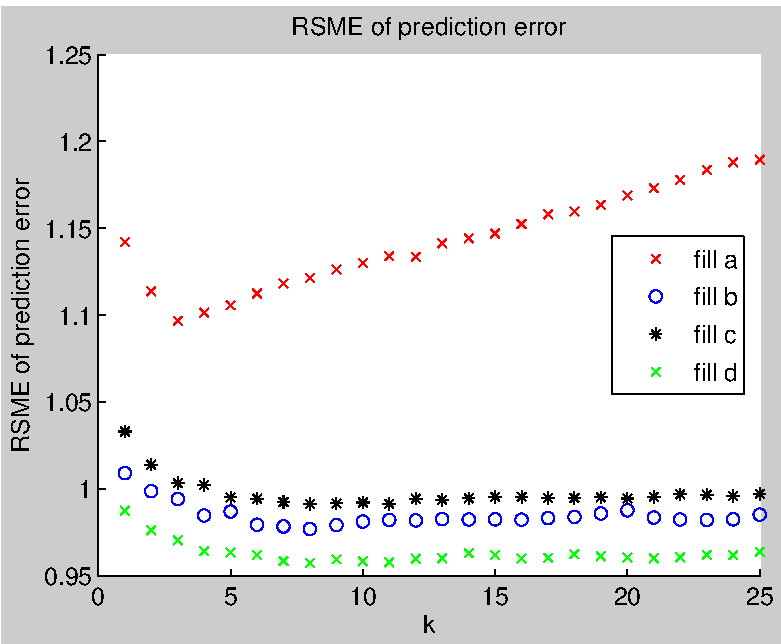
\includegraphics[width=0.7\textwidth]{rsme}
  \caption{}
\label{fig:rsme}
\end{figure}

\begin{figure}[h!]
  \centering
    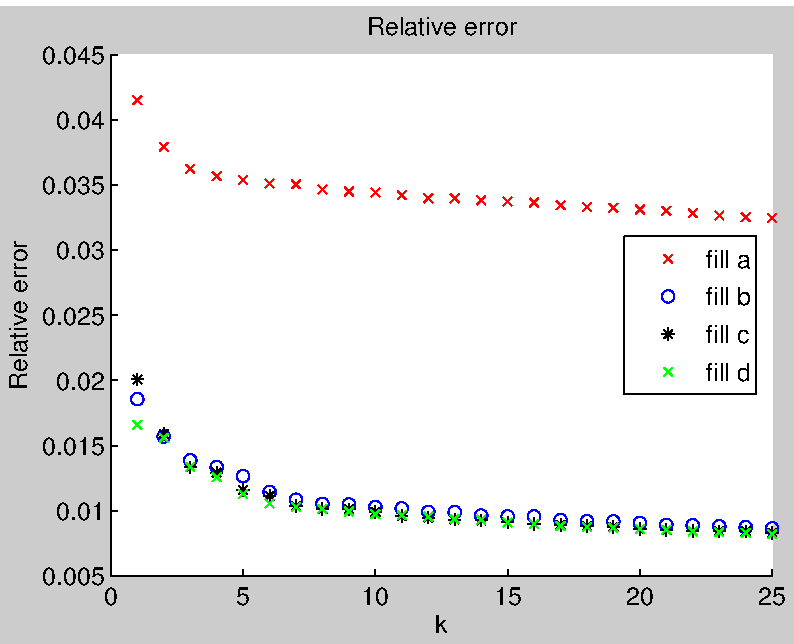
\includegraphics[width=0.7\textwidth]{relative}
  \caption{}
\label{fig:relative}
\end{figure}

The value of each singular value at each step of the iterative singular value decomposition is plotted for each of the filling methods in Figures 3-6.

\begin{figure}[h!]
  \centering
    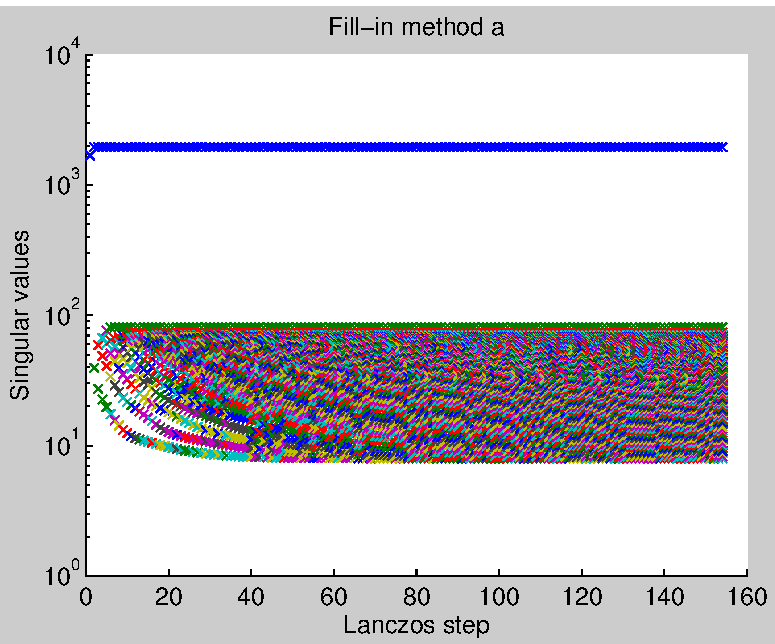
\includegraphics[width=0.7\textwidth]{sv_a}
  \caption{}
\label{fig:sv_a}
\end{figure}

\begin{figure}[h!]
  \centering
    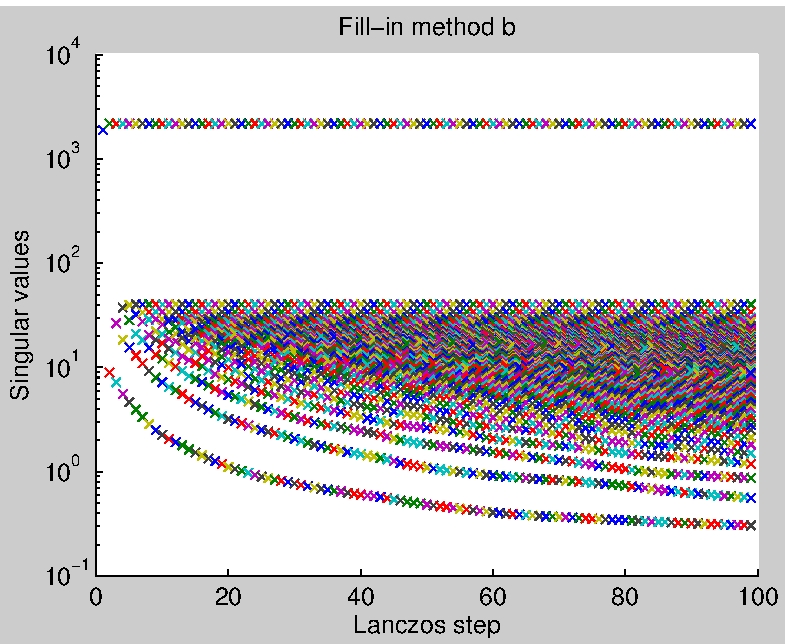
\includegraphics[width=0.7\textwidth]{sv_b}
  \caption{}
\label{fig:sv_b}
\end{figure}

\begin{figure}[h!]
  \centering
    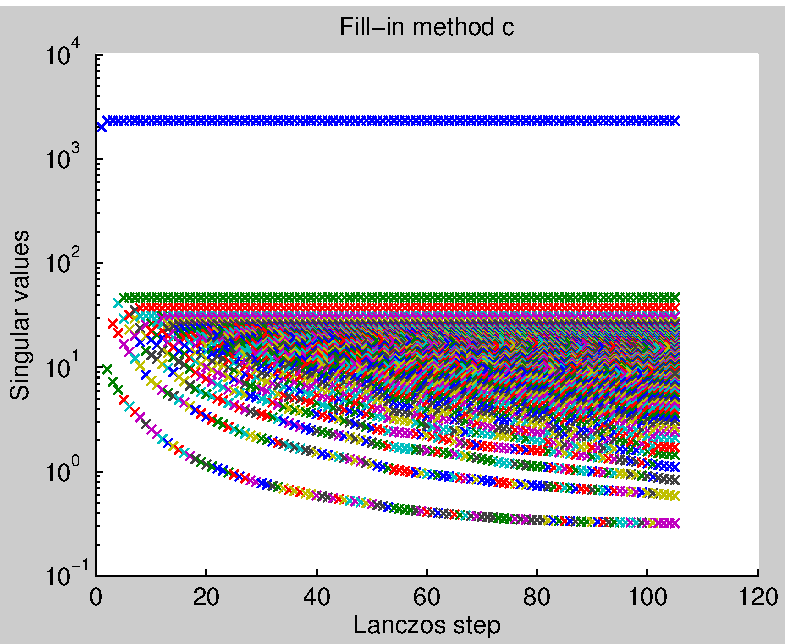
\includegraphics[width=0.7\textwidth]{sv_c}
  \caption{}
\label{fig:sv_c}
\end{figure}

\begin{figure}[h!]
  \centering
    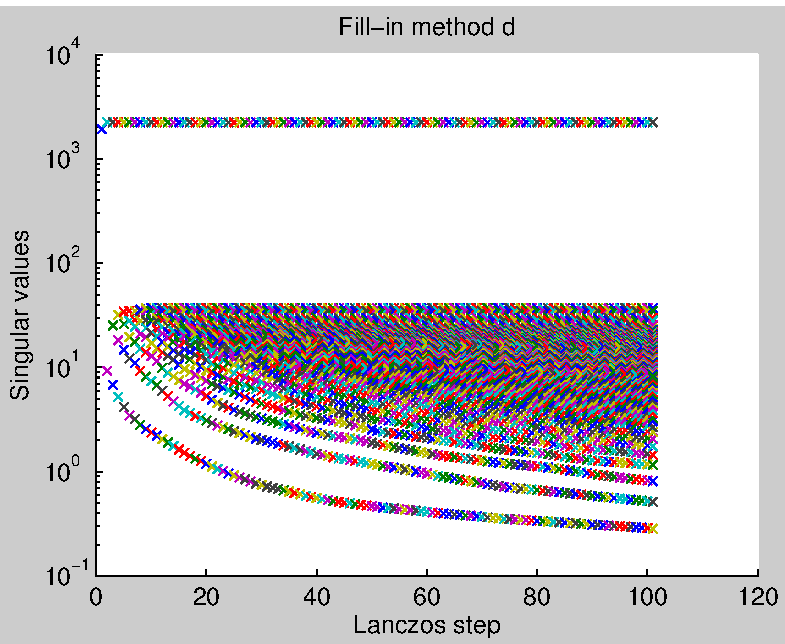
\includegraphics[width=0.7\textwidth]{sv_d}
  \caption{}
\label{fig:sv_d}
\end{figure}

The time taken to compute the SVD is plotted vs $k$ for each of the methods in Figure~\ref{fig:time}.

\begin{figure}[h!]
  \centering
    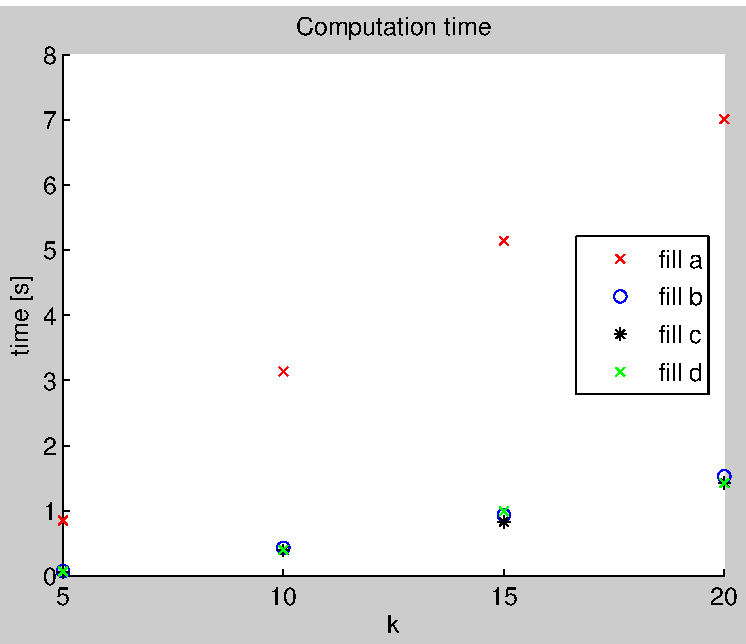
\includegraphics[width=0.7\textwidth]{time}
  \caption{}
\label{fig:time}
\end{figure}

\section{Discussion}

Looking at Figure~\ref{fig:rsme}, we see that the prediction error of the methods increases in the order: d), b), c), a). Methods b), c), and a) decrease from $k=1$ to $k =5$ and then approach a constant value. Method a)  decreases from $k=1$ to $k=3$ and then increases with $k$. These results are not surprising. As $k$ increases for the randomly filled matrix, it is using more randomly generated data which is not helpful in predicting unknown entries. The error of methods b), c), and d) include more useful information about the matrix, so they make better predictions. Method d), which uses the row and column average is the most accurate, but also requires the most computation.

Looking at Figure~\ref{fig:relative}, we see that for all methods, the  relative error between each rank-$k$ matrix and the true value of $M$ with unknown entries filled decreases with $k$. This matches the expectation that the quality of the approximation will increase with $k$. The relative error is highest for the fill method a) because the randomly filled data is not easily spanned by a set of low-rank eigenvectors.

The convergence of each singular value for each fill in method is displayed in Figures 3-6. The singular values of filling methods b), c), and d) converge more quickly than those of method a) and take approximately 50\% fewer iterations to meet the stopping criteria than method a). Most of the singular values for methods b), c), and d) are smaller than those of method a). All methods have one very large singular value that converges in only a few iterations.

Looking at Figure~\ref{fig:time}, we see that the time taken to compute the SVD has a linear relationship with $k$. This makes sense, because computing each additional singular value and set of singular vectors takes approximately the same number of operations. The filling method a) takes the most time, which  is related to the slower rate of convergence discussed earlier. The speeds of methods b), c), and d) are all comparable.

\section{Conclusions}

By all measures, the random filling of method a) performed the worst. Although filling method d) took more operations to fill in the matrix, it was the most accurate at making predictions. It would depend on the size of your matrix and your accuracy requirements, but filling in the matrix using the average of the movie rating and customer rating is likely the best option because it includes the most useful information in creating a low-rank approximation. From Figure~\ref{fig:rsme}, we see that there is no point in creating an approximation of higher order than $k=4$ or $k=5$ because it will not be any more accurate at making predictions.

\clearpage
\appendix


\section{Smetana\_Gregory\_1917370\_FINAL\_DIARY.txt}
\lstinputlisting{../Smetana_Gregory_1917370_FINAL_DIARY.txt}

\section{Smetana\_Gregory\_1917370\_FINAL.m}
\lstinputlisting{../Smetana_Gregory_1917370_FINAL.m}

\section{fill\_a.m}
\lstinputlisting{../fill_a.m}

\section{fill\_b.m}
\lstinputlisting{../fill_b.m}

\section{fill\_c.m}
\lstinputlisting{../fill_c.m}

\section{fill\_d.m}
\lstinputlisting{../fill_d.m}

\section{compute\_rsme.m}
\lstinputlisting{../compute_rsme.m}

\section{partial\_svd.m}
\lstinputlisting{../partial_svd.m}

\section{partial\_eig.m}
\lstinputlisting{../partial_eig.m}

\section{symtri\_eig.m}
\lstinputlisting{../symtri_eig.m}

%\section{Smetana\_Gregory\_1917370\_FINAL.m}
%\lstinputlisting{../Smetana_Gregory_1917370_FINAL.m}

\end{document}

